\Chapter{Tervezés}

% (8-10 oldal)
% Architektúra áttekintése

% Adatbázis
% Séma leírása

% API
% API-kat definiálni, amin majd kommunikálni lehet a backend résszel (Ez lenne a REST API megadása gyakorlatilag)
% A szinkronizációs protokollokat is definiálni kellene
% Készíteni kellene hozzá szekvencia-diagramokat

% Backend
% Az alkalmazáslogika
% Authentikáció

% Frontend
% Definiálni, hogy milyen lapokból áll majd az alkalmazás
% Leírni a játéktér megadási módját, adatszerkezeteket

% Játékszabályok ellenőrzése
% Valid lépések ellenőrzése mindkét oldalon
% Játéklogika elkészítésének tervei



% Architektúra áttekintése

A fejezet bemutatja a játéknak, mint több felhasználós, online elérhető webalkalmazásnak a tervezési folyamatát. Ez tartalmazza az alkalmazással szemben támasztott funkcionális követelményeket.

\Section{Általános funkciók}

\SubSection{Belépés az oldalra}
Az oldalra való belépéskor egy kezdőképernyő jelenik meg, ahol a játékos bejelentkezik a saját profiljába. A bejelentkezéshez szükséges megadni a felhasználónevet és a hozzá tartozó jelszót. Ha a felhasználó még nem regisztrált az oldalon, akkor a regisztráció gombra kattintva ezt is megteheti, majd ha a regisztráció sikeres volt, bejelentkezhet. A regisztrációhoz egy felhasználónév, emailcím (kétszer beírva), és jelszó megadása szükséges. Regisztráció és bejelentkezés után elérhetővé válik a személyes statisztika és megjelenés a rangsorban.

\SubSection{Új jelszó igénylése (kijelentkezve)}
Előfordul, hogy a felhasználó elfelejti felhasználónevét vagy jelszavát. Ebben az esetben lehetőség van rá, hogy új jelszót igényeljen. Ennek menete, hogy rákattint az "Elfelejtettem a jelszavamat" gombra/linkre, megadja felhasználónevét vagy emailcímét. Ezután emailt küldünk a megadott helyre. Ez az email tartalmaz egy kódot és a játékos felhasználónevét, és egy linket egy oldalra, ahol meg kell adnia az emailben küldött kódot, a felhasználónevét, és az új jelszavát kétszer. A "jelszó megváltoztatása" gombra kattintva az adatok validálódnak, és siker esetén a játékos bejelentkezhet immár új jelszóval.

\SubSection{Jelszó megváltoztatása (bejelentkezve)}
A jelszó megváltoztatására lehetőség van bejelentkezett állapotban is. Ez az egyszerűbb eset. A profil ill. beállítások oldalon a "jelszó megváltoztatása" gombra kattintva megjelenik egy űrlap, ahol meg kell adni a régi jelszót, majd az új jelszót kétszer. Az "ok" gombra kattintva az adatok validálódnak, és legközelebb már az új jelszóval léphet be a felhasználó.

\SubSection{Rangsorok, szabályzat, készítői információk megtekintése}
Ezek statikus oldalak, melyek információt biztosítanak a felhasználó számára. Interaktivitásra itt nincs lehetőség. A rangsorokat dinamikusabbá lehet tenni, ha lapozós felületet biztosítunk neki, így egyszerre csak egy kiválasztott rangsort jelenít meg.
A játék során készített statisztikák:
\begin{itemize}
	\item összes játszma (globális),
	\item összes játszma játéktípusonként (globális),
	\item személyes (a felhasználó saját statisztikái)
\end{itemize}
A felhasználó saját statisztikái és rangsorai megjelennek a profilon is. Továbbá az elérhető játékosok listáján a többi (éppen bejelentkezett) felhasználó statisztikáit is megtehetjük, amely segít annak felmérésében, hogy a megfelelő szintű játékost választhassuk ellenfélnek.

\SubSection{Hibák észlelése, jelzése}
Egy szoftver megírása során rendkívül fontos, hogy az elkészült terméket alaposan tesztelje, mielőtt élesben kiadja azt a felhasználóknak. De alapos tesztelés után is gyakori, hogy maradnak benne kisebb-nagyobb hibák, - akár figyelmetlenségből, akár hardverkülönbségek miatt, akár egy eset különlegessége miatt, stb., - amiket már csak a felhasználók tapasztalnak, vesznek észre. Olyan is lehet, hogy a szoftver kiválóan működik, de egy-egy felhasználónak akad egy jó ötlete, hogy hogyan lehetne még javítani rajta a jobb felhasználó élmény, biztonság, teljesítmény érdekében. Ezek mind-mind fontos információk a fejlesztő számára, így lehetőséget kell teremteni a felhasználóknak, hogy ezeket mind elmondhassák.

E célból kell egy olyan oldal, ahol írhatnak nekünk. Ehhez megadhatunk egy emailcímet is az oldalon, és a felhasználó írhat a saját levelező rendszeréből, de a manapság felhasználói szempontból ez már "túl sok kattintásnak" számít, így érdemesebb egy űrlapot készíteni, ahova a felhasználó leírja az észrevételeit, megnyomja a "küldés" gombot, és már kapjuk is az emailt.

\SubSection{Játék indítása}
A játék indítás oldalon több féle képpen is indíthatunk játékot. Legegyszerűbb módja, ha a kihívás listából kiválasztunk egyet. Az "elfogadás" gombra kattintva már indul is a játék.

Ha nem találunk kedvünkre való kihívást, mi magunk is létrehozhatunk egyet. Kiválaszthatjuk, hogy melyik játékkal szeretnénk játszani, és milyen szabályokkal. Létrehozás után a kihívásunk bekerül a listába, és várjuk, míg partnerünk akad. Ha menet közben meggondoljuk magunkat, és mégse szeretnénk kihívást létrehozni, lehetőség van a létrehozás megszakítására, ("megszakítás" gomb). Elfogadás után indul a játék.

\SubSection{Kihívás törlése}
Ha létrehozás után meggondoltuk magunkat, és mégsem szeretnénk a kihívásunkat (pl. nincs rá partnerünk vagy változtatnánk a szabályokon), lehetőségünk van kitörölni a listából a "kihívás törlése" gombbal. Ezután létrehozhatunk egy új kihívást, vagy elfogadhatjuk másét.
Továbbá, ha van kihívásunk a listában, és közben elfogadjuk más kihívását, a miénk automatikusan törlődik.

\SubSection{Interaktivitás bábúkkal}
Miután betöltődött a játék, a játékosok felváltva, ún. körönként játszanak. Interaktivitásra a saját körünkben van lehetőségünk a játék szabályoknak megfelelően, pl. egy bábú/karakter elhelyezése a táblán, lépés egy bábuval.

\SubSection{Játszma feladása}
Ha a vége előtt ki szeretnénk lépni a játékból, a "feladás" gombra kell kattintatunk. Ebben vége a játéknak, az ellenfél nyer, megjelennek az eredmények, majd visszatérhetünk a "játék indítása" felületre.

% ADATBÁZIS

\Section{Adatbázis}

Az adatbázisban két fontos szereplő típust, illetve azok állapotait kell nyilvántartanunk: a felhasználókat és a játékmeneteket. Habár közöttük is van kapcsolat, külön bemutatható és részletezhetők a sémáik.

\SubSection{Felhasználói adatok}
A felhasználóhoz tartozó legfontosabb információk, amiket tárolni kell, a felhasználó:
\begin{itemize}
	\item felhasználó neve,
	\item email címe,
	\item jelszavához tartozó hash kód,
	\item be van-e jelentkezve.
\end{itemize}

\SubSection{Meccsek adatai}
A meccsek adatait érdemes állapotuk, ha úgy tetszik, életciklusuk szempontjából csoportosítani. Egy meccs életének fázisai:
\begin{itemize}
	\item Kihívás:
	
	Első a kihívás, amit egy felhasználó hoz létre jelezvén, hogy játszani szeretne.
	Ez után akár meg is szűnhet, ha a játékos megszakítja (például, hogy új beállításokkal indíthasson játékmenetet), kijelentkezik, vagy ő maga egy másik kezdeményezésre jelentkezik.
	\item Aktív játékmenet:
	
	A kihívás aktív játékmenetté válik, ha egy játékos elfogad egy játékmenetet.
	\item Lejátszott meccs:
	
	A játék a végén pedig lejátszott meccs lesz. Az előző állapot minden állapotváltáskor törlődik egy kivétellel: a lejátszott meccsek adatai később sem tűnnek el, adataira statisztikai okokból később szükségünk lesz, ugyanis ezek alapján lehet felállítani a rangsorokat és az egyéni statisztikákat.
\end{itemize}
Életciklus alapján tehát megkülönböztetünk: kihívást, aktív játékmenetet, és lejátszott meccset.

Kihíváskor még nem kell sok információ: a kezdeményező játékos neve, a játék típusa, és a játék paraméterei.

A lejátszott meccseknél érdemes az azonos napon játszott, azonos típusú meccseket egy-egy rekordba összevonni, így egy-egy rekord tartalmazza, hogy egy-egy felhasználó melyik napon, milyen típusú játékban hány meccset játszott és hányat nyert meg.

Az aktív játékmenethez tartozik a játék azonosítója, típusa, a játék állása (Json sztringben), a játékosok azonosítói, nevei, és hogy éppen ki jön (aktív játékos). Habár egy játékoshoz egyszerre csak egy játékmenet tartozik, egy játékmenet több játékost is kezel egyszerre amellett, hogy vannak egyszer szereplő adattagjai is. Ennek kezelésére a játékosokat külön táblába emeltem.

Ezen szempontok alapján felvázolhatjuk adatbázisunk tábláit, melyet a \ref{fig:er-model} kép szemléltet.

\begin{figure}[!h]
	\centering
	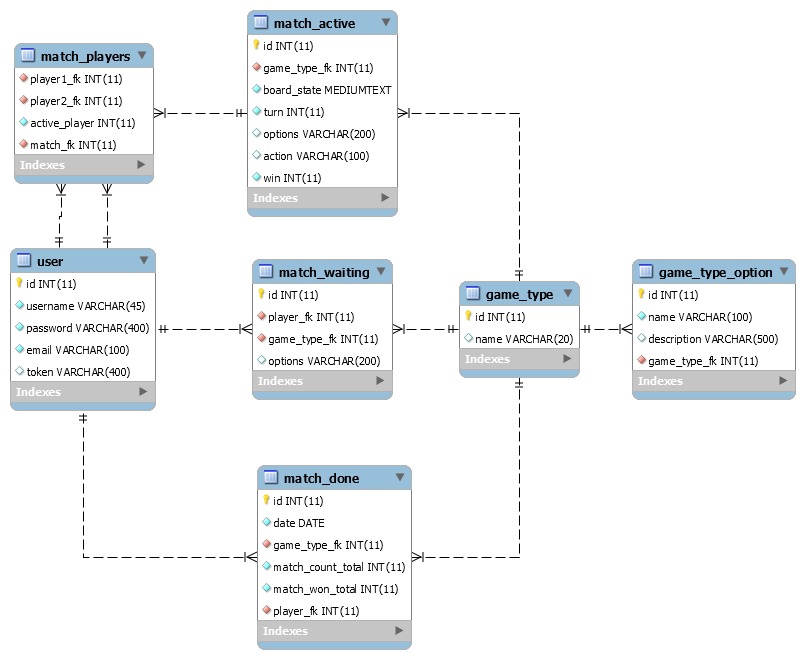
\includegraphics[width=0.9\linewidth]{kepek/online-games-er.png}
	\caption{\textit{Az adatbázis ER modellje}}
	\label{fig:er-model}
\end{figure}


% API
% API-kat definiálni, amin majd kommunikálni lehet a backend résszel (Ez lenne a REST API megadása gyakorlatilag)
% A szinkronizációs protokollokat is definiálni kellene
% Készíteni kellene hozzá szekvencia-diagramokat

\Section{REST API}

Ahhoz, hogy a frontend alkalmazásunk kommunikálni tudjon a szerverrel, egy kommunikációs felületet kell definiálnunk. Ezt a felületet interfésznek nevezzük, és itt kell megadnunk, hogy milyen kérésre mi a teendő, és hogy mi legyen a válasz. Ennek a módszernek még egy nagy előnye, hogy a komponensek, a frontend és a backend könnyen cserélhetővé válik. Feltétele csupán, hogy helyesen implementálja az interfészt.

Napjainkban nem divat a szerver oldalon generált weboldal, webkomponensek átküldése. Már csak az erőforrást (pl. egy lekért adathalmazt) küldenek át, és az oldal a frontenden generálódik. Ez az alapja a REST APInak is. Gyakran bevetett szokás ilyen környezetben, hogy a HTTP metódusokat (GET, PUT, stb.) az ún. CRUD műveletekhez rendelik. A CRUD a create (létrehozás, beszúrás), read (olvasás, lekérdezés), update (frissítés, módosítás) és delete (törlés) angol szavak kezdőbetűiből áll össze. A GET kérés megfelel a readingnek, a POST a létrehozásnak, a PUT a módosításnak, és a DELETE a törlésnek.

Az endpointokat hívhatjuk magyarul végpontoknak is. Egy endpointot tekinthetünk egy csomópontnak, vagy egy erősebb szálnak, ami segít csoportokba rendezni az elérhető szolgáltatásokat. Egyúttal megadják, hogy ezeket a szolgáltatásokat konkrétan milyen webcímen érhetjük el. Az alkalmazás az alábbi endpointokat tartalmazza:
\begin{itemize}
	\item /user/: A felhasználó ki- és beléptetését, regisztrációját, stb. segíti.
	\item /match/: A játék elindítást kezeli.
	\item /fiveinarow/: A malom játékot vezérli.
	\item /checkers/: A dáma játékot vezérli.
	\item /stats/: Lekérdezi és összeállítja a statisztikákat.
\end{itemize}

%TODO CIMKÉKET ELLENŐRIZNI!

% USER

\SubSection{/user}
\texttt{POST}: Validálja a felhasználó által megadott értékeket, és elmenti az új profilt az adatbázisba.
Siker esetén megerősítő üzenetet küld a mentés sikeréről.
Sikertelen művelet esetén hibaüzenetet küld a felhasználónak (\ref{lst:user-save} ábra).

\lstinputlisting[caption={\textit{/user POST kérés és válasz minta}}, label={lst:user-save}]{kodok/api/user-save.json}

\texttt{PUT}: Validálja a felhasználó által megadott értékeket, és elmenti az új értékeket az adatbázisba. A felhasználó egyelőre csak a jelszavát tudja megváltoztatni.
Siker esetén megerősítő üzenetet küld a mentés sikeréről.
Sikertelen művelet esetén hibaüzenetet küld a felhasználónak (\ref{lst:user-update} ábra).

\lstinputlisting[caption={\textit{/user PUT kérés és válasz minta}}, label={lst:user-update}]{kodok/api/user-update.json}

\texttt{DELETE}: Validálja a felhasználó által megadott értékeket, (a törléshez szükség van a jelszó megadásához), majd törli a felhasználót az adatbázisból. Gyakran bevett szokás, hogy a felhasználó rekordját valójában nem törlik ki, hanem csak egy plusz mezőben átírják az állapotát aktívról töröltre. Ez főként olyan alkalmazásoknál jelentős, ahol fontos a visszakereshetőség biztosítása akár több évre visszamenőleg is, pl. bankoknál. Esetünkben a felhasználó teljesen törlésre kerül.
Siker esetén megerősítő üzenetet küld a törlés sikeréről. (Egyúttal illik kiléptetni a felhasználót).
Sikertelen művelet esetén hibaüzenetet küld a felhasználónak (\ref{lst:user-delete} ábra).

\lstinputlisting[caption={\textit{/user DELETE kérés és válasz minta}}, label={lst:user-delete}]{kodok/api/user-delete.json}

\SubSection{/user/authenticate}
\texttt{POST}: Validálja a felhasználó nevét és jelszavát.
Siker esetén elküldi az azonosító tokent.
Sikertelen művelet esetén hibaüzenetet küld a felhasználónak. (\ref{lst:user-authenticate} ábra).

\lstinputlisting[caption={\textit{/user/authenticate kérés és válasz minta}}, label={lst:user-authenticate}]{kodok/api/user-authenticate.json}

\SubSection{/user/forgottenpassword}
\texttt{POST}: Validálja az adatokat, (ellenőrzi, hogy a felhasználó létezik-e az adatbázisban), majd küld egy megerősítő emailt a felhasználó címére, a linkkel, amin tovább haladva megadhatja új jelszavát.
Siker esetén elküldi, hogy a validáció sikeres. (Csak ez után jelenik meg az űrlap az új jelszó megadásához).
Sikertelen művelet esetén hibaüzenet küld a felhasználónak (\ref{lst:user-forgottenpassword} ábra).

\lstinputlisting[caption={\textit{/user/forgottenpassword kérés és válasz minta}}, label={lst:user-forgottenpassword}]{kodok/api/user-forgottenpassword.json}

% MATCH

\SubSection{match}
\texttt{GET}: Ellenőrzi a felhasználót, majd lekérdezi és válaszként elküldi a várakozó meccsek (kihívások) adatainak listáját (\ref{lst:match-list} ábra).

\lstinputlisting[caption={\textit{/match/list kérés és válasz minta}}, label={lst:match-list}]{kodok/api/match-list.json}

\texttt{POST}: Inicializál egy új kihívást és elmenti az adatbázisba. (Emellett gondoskodni kell róla, hogy a többi felhasználó számára is megjelenjen az új kihívás). A művelet végén visszaküldi a mentés sikerességét.
Sikertelen művelet esetén hibaüzenet küld a felhasználónak (\ref{lst:match-create} ábra).

\lstinputlisting[caption={\textit{/match/create kérés és válasz minta}}, label={lst:match-create}]{kodok/api/match-create.json}

\texttt{DELETE}: Kitöröl egy kihívást és elmenti az adatbázisba. (Emellett gondoskodni kell róla, hogy a többi felhasználó számára is eltűnjön az új kihívás).
Siker esetén elküldi, hogy a törlés sikeres.
Sikertelen művelet esetén hibaüzenet küld a felhasználónak (\ref{lst:match-delete} ábra).

\lstinputlisting[caption={\textit{/match/delete kérés és válasz minta}}, label={lst:match-delete}]{kodok/api/match-delete.json}

\SubSection{match/start}
\texttt{POST}: Akkor hívódik meg, amikor egy játékos elfogad egy kihívást. Megkapja az ezidáig várakozó játszma és a játékos azonosítóját. Lekéri a várakozó játék adatait, létre hozz egy aktív játszmát, amit elment az adatbázisban is, majd törli a várakozó játékot. Ha bármelyik játékosnak volt aktív kihívása, azt törli az adatbázisból.
Sikeres mentés esetén megerősítésképpen visszaküldi a meccs adatait tartalmazó objektumot.
Sikertelen művelet esetén hibaüzenetet küld a felhasználónak (\ref{lst:match-start} ábra).

\lstinputlisting[caption={\textit{/match/start kérés és válasz minta}}, label={lst:match-start}]{kodok/api/match-start.json}

\texttt{GET}: Megkapja a játékos azonosítóját és ellenőrzi, hogy a játékos szerepel-e aktív játékban. Ha a válasz igen, elküldi a meccs adatait tartalmazó objektumot. Ha még nincs játékban, az objektum értéke \texttt{null} (\ref{lst:match-checkstart} ábra).

\lstinputlisting[caption={\textit{/match/checkstart kérés és válasz minta}}, label={lst:match-checkstart}]{kodok/api/match-checkstart.json}

% FIVE IN A ROW

\SubSection{/fiveinarow/action}
\texttt{POST}: Mikor a soron következő játékos elvégzi a lépést (vagy ezzel egyenértékű cselekvést, pl. elhelyez egy csapdát), megkapja a meccs állását és a cselekvés adatait. Ezek segítségével ellenőrzi a lépés helyességét és hogy nyert -e a játékos, majd elmenti az adatbázisba.
Siker esetén elküldi a kiértékelés eredményét, hogy volt-e nyerés, és sikerült -e a mentés. Ha nem sikerült, hibaüzenetet küld (\ref{lst:fiveinarow-action} ábra).

\lstinputlisting[caption={\textit{/fiveinarow/action kérés és válasz minta}}, label={lst:fiveinarow-action}]{kodok/api/fiveinarow-action.json}

\SubSection{/fiveinarow/checkaction}
\texttt{GET}: Rendszeres időközönként meghívódik annak ellenőrzésére, hogy az ellenfél lépett-e már. Megnézi, hogy az adatbázisban tárolt kör száma nagyobb -e, mint a kapotté. Ha igen, visszaküldi a meccs objektumot, ha nem, akkor az objektum \texttt{null} (\ref{lst:fiveinarow-checkaction} ábra).

\lstinputlisting[caption={\textit{/fiveinarow/checkaction kérés és válasz minta}}, label={lst:fiveinarow-checkaction}]{kodok/api/fiveinarow-checkaction.json}

\SubSection{/fiveinarow/timeout}
\texttt{POST}: Egy játékos inaktivitása esetén kap egy jelzést, majd a kört átadja az ellenfélnek (\ref{lst:fiveinarow-timeout} ábra).

\lstinputlisting[caption={\textit{/fiveinarow/timeout kérés és válasz minta}}, label={lst:fiveinarow-timeout}]{kodok/api/fiveinarow-timeout.json}

\SubSection{/fiveinarow/giveup}
\texttt{POST}: Megkapja a felhasználó azonosítóját és a meccs objektumot, és elmenti az eredményt a meccs objektumba. Visszatérési értéke a mentés sikeressége (\ref{lst:fiveinarow-giveup} ábra).

\lstinputlisting[caption={\textit{/fiveinarow/giveup kérés és válasz minta}}, label={lst:fiveinarow-giveup}]{kodok/api/fiveinarow-giveup.json}

% STATS

\SubSection{stats/global}
\texttt{GET}: Lekéri a szükséges adatokat az adatbázisból, majd összeállítja és visszaküldi a rendezett ranglistát (\ref{lst:stats-global} ábra).

\lstinputlisting[caption={\textit{/stats/global kérés és válasz minta}}, label={lst:stats-global}]{kodok/api/stats-global.json}

\SubSection{stats/globalbygametype}
\texttt{GET}: Lekéri a szükséges adatokat az adatbázisból, majd összeállítja és visszaküldi a rendezett ranglistát (\ref{lst:stats-globalbygametype} ábra).

\lstinputlisting[caption={\textit{/stats/globalbygametype kérés és válasz minta}}, label={lst:stats-globalbygametype}]{kodok/api/stats-globalbygametype.json}

\SubSection{stats/personal}
\texttt{GET}: Megkapja a felhasználó azonosítóját, majd lekéri a szükséges adatokat az adatbázisból, majd összeállítja és visszaküldi a rendezett ranglistát (\ref{lst:stats-personal} ábra).

\lstinputlisting[caption={\textit{/stats/personal kérés és válasz minta}}, label={lst:stats-personal}]{kodok/api/stats-personal.json}


\Section{Komponensek}

A készülő alkalmazás felépítésének tervezéskor két szempontot érdemes figyelembe venni: az egyik a HTTP kliens-szerver architektúra, a másik az MVC architektúra.

\SubSection{HTTP kliens-szerver architektúra}
Minden egyes HTTP protokollt használó kommunikáció esetében van egy kérés és egy válasz. Az ügyfél böngészője egyetlen kérést intéz a szerverhez, amely alapján a szerver meghatározza a kért erőforrást és válaszul visszaküldi a kért állomány tartalmát. Ezt követően az ügyfél böngészője értelmezi a választ és megjeleníti a kapott tartalmat. A kérés az igényelt erőforráson kívül más információkat is tartalmaz. Ilyen információ például az ügyfél böngészőjének a típusa. A kérés általában sima szöveges információ, a válasz pedig lehet szöveg, illetve bináris adat is \cite{java-web-tech}.

\SubSection{MVC architektúra}
%Elsőként a Xerox írta le a 1980-as évek végén, azóta más GUI alkalmazások készítésére alkalmas környezet is átvette ezt a modellt.
Az alapgondolat az, hogy egy alkalmazás adatait, ezek megjelenítését, illetve ezek kapcsolatát három önálló egységre bontja szét, amelyek nevei: Model (modell), View (megjelenítés), illetve Controller (vezérlés). A szétbontás célja az, hogy rugalmas alkalmazásokat készíthessünk, például kicserélhessük az adatok megjelenítését a többi rész változtatása nélkül.
% Egyre szélesebb körben terjednek el a mobiltelefonok, PDA-k, amelyek internetkapcsolat segítségével alkalmassá váltak tartalom megjelenítésére. Csakhogy ezek mérete különböző, így ugyanazon tartalmat más és más formában kell megjeleníteni. Gyakorlatilag úgy kell elkészíteni az alkalmazást, hogy ez képes legyen a kommunikációs eszköznek megfelelő tartalmat előállítani. Ennek megvalósítása szükségessé tette az alkalmazásoknak három részre bontását: modell (Model), megjelenítés (View) és vezérlés (Controller).

A modell részt rendszerint az adatok és ezek elérési logikája képezi. Ez a rész az, amely a legritkábban változik. A vezérlés a közvetítő a modell és a megjelenítés között, amely vagy aktualizálja a modellt, vagy pedig egy új nézetet jelenít meg. A megjelenítés pedig sokféle lehet. Ha időközben ugyanazon alkalmazáshoz egy új kommunikációs eszközt akarunk csatlakoztatni, akkor csak az ennek megfelelő megjelenítési réteggel kell kiegészíteni az alkalmazást. Tehát ennek a tervezési mintának a betartása is nagymértékben hozzájárul az alkalmazások rugalmasságának növeléséhez.

%A [hivatkozás] ábra egy űrlap kitöltésének MVC architektúráját szemlélteti, amely során az űrlapadatok a megjelenítési rétegből átkerülnek a vezérlési réteghez, ahol megtörténik az adatok ellenőrzése. Hibás adatok esetén a vezérlés új megjelenítést generál, amely figyelmezteti a felhasználót a hibákra. Ha helyesek voltak az adatok, eltárolódnak a modell rétegben. Egy másik lehetséges forgatókönyv az, amikor az űrlap bizonyos adatok lekérdezését valósítja meg. Ebben az esetben a vezérlés feladata az adatok lekérése a modell rétegből és az ezt tartalmazó új nézetet előállítása és eljuttatása az ügyfélhez.

Az MVC tervezési minta először grafikus interfészek (desktop alkalmazások) készítésével kapcsolatban jelent meg, később alkalmazták például webalkalmazások architektúrájaként is. Webalkalmazások esetében a vezérlési réteg feladata a kérések feldolgozása és továbbítása a megfelelő komponens fele. Így a vezérlési rész felügyeli az alkalmazást, a modell pedig az alkalmazás állapotát tárolja. Összefoglalva, a következő előnyökkel rendelkezik egy MVC architektúrájú alkalmazás:
\begin{itemize}
	\item Lehetővé teszi több, különböző megjelenítés illesztését ugyanazon modellhez.
	\item Szétválasztja az alkalmazás üzleti logika, adatelérés, illetve megjelenítés részeit, amely növeli az alkalmazás rugalmasságát \cite{java-web-tech}.
\end{itemize}

\SubSection{Szerkezet összegzés}

A két fent említett szerkezetet alkalmazva az alábbi alkalmazás vázat kapjuk:

A HTTP protokollnak megfelelően először definiáljuk a klienst (fronendet) és a szervert (backendet), majd ezekben helyezzük el az MVC komponenseket. Magától értetődő, hogy a View teljes mértékben a frontend része, a Model, - ami gyakorlatilag az adatbázist és adat kezelő logikát jelenti-, pedig a backendé. Az érdekes rész a Controller, mivel esetünkben a lépéseket és az űrlap adatait mindkét oldalon ellenőrizni kell, így a frontend és a backend is tartalmaz üzleti logikát (\ref{fig:mixed-arch}. ábra).
\begin{figure}[!h]
	\centering
	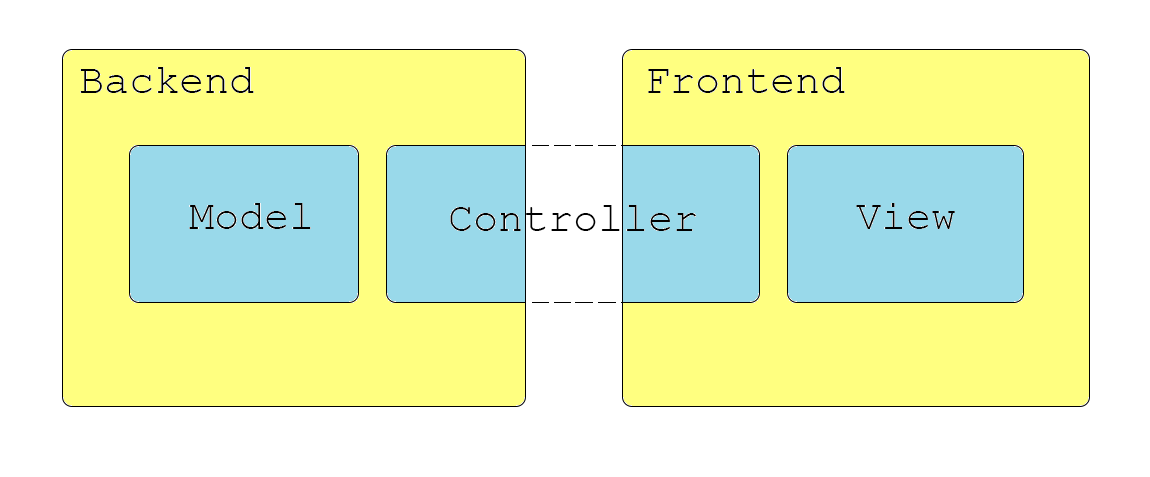
\includegraphics[width=0.5\linewidth]{kepek/mixed-arch.png}
	\caption{\textit{Az MVC megoszlása a backend és a frontend között}}
	\label{fig:mixed-arch}
\end{figure}

\Section{Backend felépítése}

\SubSection{Réteges architektúra}

A \textit{backend} vagy más néven szerver oldali alkalmazás, egy kiszolgáló alkalmazás, amelyet (első sorban) webböngészővel érhetünk el. Feladata a kliens (frontend) által küldött adatok feldolgozása, majd a megfelelő válasz, ill. erőforrás visszaküldése. Mint általában a szoftvereknél, a szerver alkalmazást is érdemes jól elkülöníthető rétegekre bontani, melyet a \ref{fig:server-layers} ábra szemléltet.

\begin{figure}[!h]
	\centering
	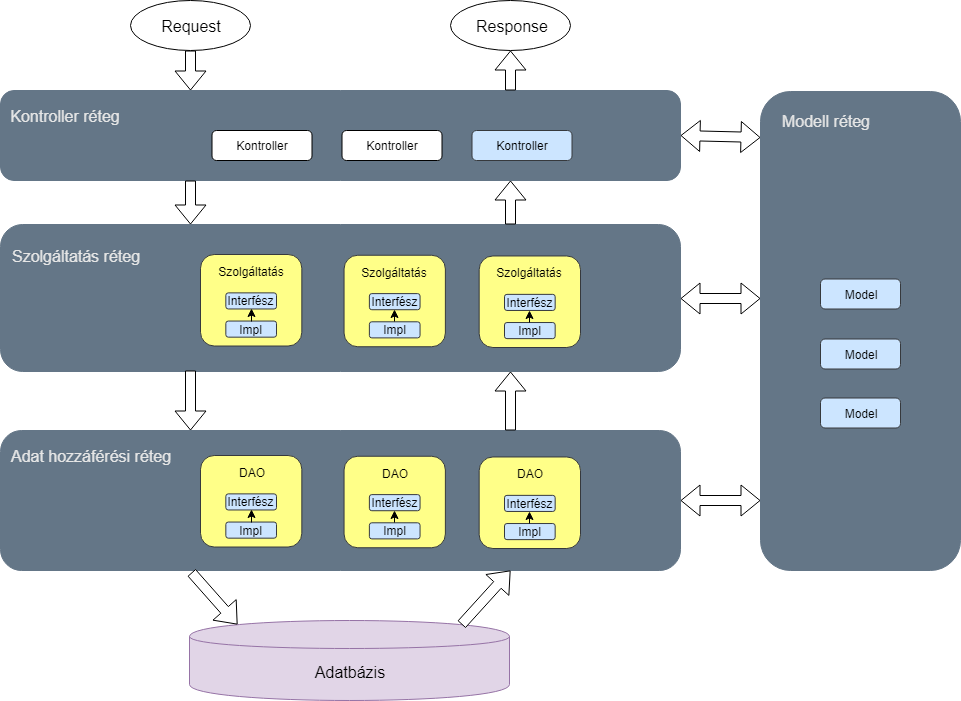
\includegraphics[width=0.9\linewidth]{kepek/server-layers-colored.png}
	\caption{\textit{Szerver rétegek}}
	\label{fig:server-layers}
\end{figure}

Az első réteg, a web réteg, vagy más néven kontroller (controller) réteg. Mikor a böngésző a korábban már definiált API alapján elküld egy kérést a szervernek, az alkalmazás megkeresi a hívás címén keresztül a megfelelő kontrollert. A kontrollerek feladata a kérések fogadása és a válaszok visszaküldése.  A kettő között azonban szükség van az adatok feldolgozására, melyet már a következő szinten, a szolgáltatás (service) rétegben végzünk. Ennek szolgáltatásait a kontrollerek veszik igénybe. Az adat feldolgozás során gyakran van szükség az adatok tartós tárolására és karban tartására, tehát szükség van egy adatbázisra is. Ahhoz, hogy a szolgáltatások és az adatbázis között létrejöhessen a kapcsolat, be kell hát vezetnünk még egy szintet, ez lesz az adat hozzáférési réteg (persistence). Feladata, a kapcsolat kiépítése az alkalmazás, majd az adatbázis között és elküldeni az adatbázisnak az elvégzendő műveleteket, és fogadni annak eredményét. Van még egy réteg, mely hierarchiában nem ennyire meghatározható, hiszen bármely réteg szükség szerint hozzáférhet, ez pedig a modell réteg. Ebben egyszerű objektumokat találunk, melyeknek a szerepe, hogy meghatározzák az objektumok struktúráját.

Az MVC architektúra előnyei között említettük a rugalmasságot, vagyis a komponensek cserélhetőségét. A szerver esetében is szokás ilyen szempont szerint tervezni. Ennek a legfontosabb eszközei az interfészek, melynek segítségével a komponensek bármikor cserélhetőek úgy, hogy az alkalmazást csak egyetlen ponton, a példányosítás megadásakor kell módosítani. Ezek a pontokat rendszerint annotációk, (mára ez az elterjedtebb), vagy xml fájlok segítségével konfiguráljuk.

\SubSection{Kontrollerek meghatározása}
Mint láthattuk az alkalmazásnak sok kisebb funkciója van külön fajta kérésekkel, de felesleges lenne minden kéréshez külön külön kontrollert fenntartani, így érdemes jellegük szerint csoportosítani őket, és néhány kontrollerrel kezelni őket. Így az alábbi kontrollereket kapjuk:
\begin{itemize}
	\item felhasználói (továbbiakban UserController),
	\item meccs (továbbiakban MatchController),
	\item amőba (továbbiakban FiveInARowController),
	\item dáma (továbbiakban CheckersController).
\end{itemize}
Ezek mélyebb ismertetését a következőkben olvashatjuk.

\subsubsection{UserController}
A UserController fő feladata magával a felhasználó személyével kapcsolatos kérések kezelése. Ide tartozik
\begin{itemize}
	\item a regisztráció,
	\item a bejelentkezés,
	\item a kijelentkezés,
	\item jelszó megváltoztatása,
	\item a elfelejtett jelszó kezelése,
	\item és a felhasználó törlése.
\end{itemize}

\subsubsection{MatchController}
A MatchController, ahogy a neve is sugallja a meccsek kezelésével kapcsolatos kéréseket dolgozza fel. Ennek feladata
\begin{itemize}
	\item a kihívások (meccs kezdeményezések) létrehozása,
	\item törlése,
	\item a kihívások listájának lekérdezése,
	\item és az aktív játékmenet létrehozása elfogadáskor.
\end{itemize}

\subsubsection{FiveInARowController}
Az amőba kontrollere értelem szerűen már a megkezdett, amőba játéktípusú meccs kéréseit kezeli. Ezek az alábbiak:
\begin{itemize}
	\item az aktív játékos lép,
	\item lépett -e az ellenfél,
	\item lejárt a lépéshez megengedett idő (timeout),
	\item játék feladása
\end{itemize}

\subsubsection{CheckersController}
Hasonló jellegű kéréseket kell teljesítenie, mint egyéb típusú játékok esetén, a játék sajátosságai miatt minden játéktípusnak külön kontrollerre és metódusokra van szüksége.

\subsubsection{StatsController}
Feladata a lejátszott meccsek adataiból összeállítani statisztikákat, rangsorokat, majd ezt az adathalmazt elküldeni a frontendnek.


% MODEL OSZÁLYOK

\SubSection{Modell osztályok}

Miután felvázoltuk az adatbázist és meghatároztuk az eltárolandó adatot, ez alapján rögzíthetjük a szerver oldalon szükséges modell osztályokat, amelynek a következőket kell tartalmaznia: azonosító, felhasználónév, a jelszó hashkódja, emailcím.


\subsubsection{Felhasználó modell}
Elsőként a User (felhasználó) osztállyal kell foglalkoznunk, ami minden más osztállyal kapcsolatban áll. (\ref{lst:user} ábra).

\lstinputlisting[caption={\textit{A felhasználó modell osztály adattagjai}}, label={lst:user}]{kodok/model/user.json}

\subsubsection{Kihívás modell}
A kihívás modell a várakozó meccseket reprezentálja, amelyeket a felhasználók hoznak létre. Tartalma a kihívás azonosítója, a felhasználó azonosítója, a játék típusa, és egy tömbben a kiválasztott beállítások. (\ref{lst:match_waiting} ábra).

\lstinputlisting[caption={\textit{A kihívás modell osztály adattagjai}}, label={lst:match_waiting}]{kodok/model/match_waiting.json}

\subsubsection{Aktív meccs modell}
Az aktív meccsek adatmezői a meccs, a játékosok azonosítói, a soron következő játékos száma (1 vagy 2), a játék típusa, a játék állása, és hogy hanyadik körnél tartunk (\ref{lst:match_active} ábra). Mivel az adatbázisban az aktív meccsek játékosait külön táblába kellett emelnünk, a könnyebb konverzió érdekében ezeket a modellben is egy külön osztályba emeljük ki. A játék állását az adatbázisba mindig sztringként tároljuk el, ám a könnyebb kezelhetőség és az ellenőrzések érdekében objektumként is szükségünk van rá, ezért mindkét formában benne kell lennie.

\lstinputlisting[caption={\textit{Az aktív meccs modell osztály adattagjai}}, label={lst:match_active}]{kodok/model/match_active.json}

\subsubsection{Játékosok modell}
A játékosok modell szerkezete egyszerű, csak három azonosítót tartalmaz: a két résztvevő és a soron következő játékos számát (\ref{lst:players} ábra).

\lstinputlisting[caption={\textit{A játékosok modell osztály adattagjai}}, label={lst:players}]{kodok/model/players.json}

\subsubsection{Játékállás modell}
Mivel a különböző játékokhoz különböző táblák tartozhatnak, így minden típusra érdemes külön modell osztályt írni.

Az amőba játékállás reprezentálását már a \ref{board-repr} pontban tárgyaltuk. Az így megadott mátrixban tárolt objektum halmazt a \ref{lst:fields} ábra szemlélteti.

\lstinputlisting[caption={\textit{A játékállás modell osztály adattagjai}}, label={lst:fields}]{kodok/model/fields.json}

\subsubsection{Lejátszott játék modell}
%TODO match done pontosítani!!!
A statisztikák generálásához szükséges megőriznünk a játékeredményeket (\ref{lst:match_done} ábra).

\lstinputlisting[caption={\textit{A lejátszott játék modell osztály adattagjai}}, label={lst:match_done}]{kodok/model/match_done.json}

\subsubsection{Felsorolások}
A sztringek kezelése kissé nehézkesebb, mint a számoké, ugyanakkor érdemes rögzíteni, hogy melyik szám melyik játékra utal. Ezért a \texttt{játéktípusokat}, és az egyéni szabályok beállításait érdemes enumokban tárolni.

Mivel a különböző játéktípusokhoz különböző egyéni szabályok tartozhatnak, így a \texttt{játékszabályoknak} játéktípusonként egy enum osztályt kell készítenünk.

És mivel a pálya mezőinek is kötött, hogy milyen értékeket lehet adni, így játéktípusonként szükségünk lesz egy-egy \texttt{érték} enumra is.

\Section{Frontend alkalmazás részei}

A \textit{frontend} ez esetben a webböngészőben futó JavaScript alkalmazást jelenti. A következő szakaszokban ezen alkalmazás részeinek és működésének a bemutatására kerül sor.

\SubSection{Komponensek}
A frontend a korábban megfogalmazott igényeket figyelembe véve az alábbi oldalakból fog állni:
\begin{itemize}
	\item bejelentkezés (főoldal),
	\item regisztráció,
	\item elfelejtett jelszó,
	\item bemutatkozás,
	\item játékszabályok,
	\item használati feltételek,
	\item profil,
	\item beállítások,
	\item játék indítás,
	\item aktív játéktér,
	\item statisztikák.
\end{itemize}
A játéktér kivételével minden oldalon megjelenik egy menüsor, ami segítheti a felhasználót a navigációban. Mivel bizonyos funkciókhoz bejelentkezés szükséges, így a menüsornak is alkalmazkodni kell a felhasználó állapotához. Ezt tokenek segítségével valósítjuk meg, melyről később bővebben is esik szó.

Továbbá a játéktérre csak a játék indítás oldalon keresztül lehet eljutni, az elfelejtett jelszóhoz és a regisztrációhoz pedig lesz egy-egy link a főoldalon, így a menüsorban ezek nem jelennek meg. Ha játéktérre a megengedettől eltérő módon lépne be valaki, a hiányzó adatok és ellenfél híján hibát kapnánk. Megoldásként, bármilyen hiba esetén a felhasználót átirányítjuk a játék indítás oldalra.

Vendég felhasználóként (tehát bárki számára) csak az alábbi linkek érhetők el:
\begin{itemize}
	\item bejelentkezés,
	\item regisztráció,
	\item elfelejtett jelszó,
	\item bemutatkozás,
	\item játékszabályok,
	\item használati feltételek.
\end{itemize}

\subsubsection{Bejelentkezés}
Ez a főoldal, ami néhány mondatban köszönti a vendég felhasználót az oldalról, aki itt bejelentkezhet az alkalmazásba egy űrlapon keresztül.
Sikeres bejelentkezés esetén megjeleníti a felhasználó profilját és a menüben megjelenik a kijelentkezés gomb.
További linkek az oldalon:
\begin{itemize}
	\item regisztráció,
	\item elfelejtett jelszó.
\end{itemize}
Elfelejtett jelszó esetén újabb űrlap jelenik meg, amivel a felhasználó elküldheti felhasználónevét és/vagy jelszavát.


\subsubsection{Regisztráció}
Egy formot jelenít meg, amelyben a felhasználó megadhatja a regisztrációhoz szükséges adatokat. Elküldés után a felhasználó visszajelzést kap a regisztráció sikerességéről.

\subsubsection{Elfelejtett jelszó}
Ez az oldal akkor jelenik meg, ha az elfelejtett jelszó kapcsán küldött emailben található linkre kattintunk. Itt a felhasználónak egy újabb űrlapon kétszer meg kell adnia az új jelszót. Elküldés után a mentés sikerességéről értesítést jelenít meg.

\subsubsection{Bemutatkozás, Játék szabályok, Használati feltételek}
Általános, tájékoztató jellegű leírások. Statikus adatokat megjelenítő oldalak, akció nincs.

\subsubsection{Profil}
(Felhasználó)név szerint köszönti a bejelentkezett felhasználót. Megjelenik egy menü a további lehetőségekről, és akár néhány személyes információ is (pl. avatar, nyerési arány, egy véletlen szerű vicc, stb).

\subsubsection{Játék kiválasztása}
Itt két fontos opciót találhatunk, amely a képernyőt két részre osztja.

Az egyik oldalon táblázat formájában böngészhetünk a meccsek közül. Ezek soronként tartalmazzák a kihívó játékos nevét, a játék típusát, és a lehetséges szabálymódosításokat. Ha találunk kedvünkre való meccset, kiválasztva azt, majd az "ok" gombra kattintva kezdhetjük is a játékot.

Ha egyik felkínált lehetőség sem tetszik, tekintsünk a másik oldalra, ahol magunk is létrehozhatunk egy meccset. Ezen az oldalon megjelenik egy menü a játéktípusok felsorolásával és a választható szabályváltoztatásokkal. Ha minden opciót beállítottunk, az ehhez az oldalhoz tartozó "ok" gombbal hozzáadhatjuk kihívásunkat az említett kihívás listához. Egy felhasználó egyszerre csak egy kihívást kezdeményezhet, ilyenkor a kihívás hozzáadása gomb tiltásra kerül. Saját kihívásunkat a lista más színnel jelöli, mint a többit. Saját kihívásunkat kijelölve megjelenik egy törlés gomb. 

Innen kezdve 3 lehetőségünk lesz:
\begin{itemize}
	\item várunk egy ellenfélre,
	\item töröljük a kihívásunkat, (majd létrehozhatunk egy másik kihívást),
	\item választunk egy meccset a listából, (ebben az esetben az általunk létrehozott meccs törlődik).
\end{itemize}

\subsubsection{Játéktér}
Megjelenik a játéktér a játéktípushoz tartozó interaktív elemekkel.

A játék végén (ha a játék szabályosan véget ért vagy az egyik játékos feladta) megjelenik az eredmény-hirdetés. A tovább gombra kattintva a Játék indítása oldalra visz.

\subsubsection{Rangsorok}
Itt jelennek meg a játék során készített statisztikák:
összes játszma száma (globális)
játszmák száma játéktípusonként (globális)
nyerési arány összesen (felhasználónként)
nyerési arány játéktípusonként (felhasználónként)
A statisztikák elkészíthetők úgy is, hogy egyszerre csak egy (kiválasztott) listát mutasson.

\subsubsection{Beállítások}
A felhasználó bizonyos mértékig személyre szabhatja az alkalmazást. Egyelőre csak a jelszavát tudja majd megváltoztatni, de később implementálni lehet pl. avatar képek feltöltését, szín séma megváltoztatását, stb. A változások mentése előtt meg kell adni az érvényes jelszót.

A mentések sikerességéről visszajelzést jelenít meg (sikeres vagy hibaüzenet).

\subsubsection{Kijelentkezés}
A kijelentkezés gombra kattintva a felhasználó kijelentkezhet az alkalmazásból. Az alkalmazás ekkor törli a bejelentkezéskor kapott tokent, majd átirányítja a felhasználót a bejelentkezés oldalra. Külön oldal nem tartozik hozzá.

\Section{Alkalmazás logika}

A komponenseket ugyan megterveztük, de rengeteg kérdés merül fel azzal kapcsolatban, hogy hogyan fognak ezek a komponensek együtt működni. Hogyan szinkronizáljuk a játék menetét, hogy mindkét játékos (lehetőleg) valós időben lássa a másik lépéseit? Szinkronizáljuk a böngészők eseményeit? Egyáltalán milyen feladatok merülnek fel, amikre a tervezés legelején nem gondolna az ember? Nézzük sorban!

\SubSection{A backend és a frontend kapcsolata}
Az első és legfontosabb kérdés, hogy hogyan fogja látni az egyik böngésző, hogy mi történik a másikban, pl. ha lép a játékos, hogyan jut át az információ? Ahogy egy pincér egy jó étteremben, a szerver (pincér) kiszolgál, a kliens pedig rendel. Tehát minden eseményt vagy kérést a klienst küld el a szervernek, ill. ha a szerverhez befut egy információ, a szerver nem tolakodik a böngészőhöz, hogy átadja az információt, sőt azt sem tudja, hogy a frontendnek szüksége van rá. Ezért az alkalmazásban minden kommunikációt a frontend kezdeményez.

A komponenseket ugyan megterveztük, de rengeteg kérdés merül fel azzal kapcsolatban, hogy hogyan fognak ezek a komponensek együtt működni. Hogyan szinkronizáljuk a játék menetét, hogy mindkét játékos (lehetőleg) valós időben lássa a másik lépéseit? Szinkronizáljuk a böngészők eseményeit? Egyáltalán milyen feladatok merülnek fel, amikre a tervezés legelején nem gondolna az ember? Nézzük sorban!

\SubSection{A backend és a frontend kapcsolata}
Az első és legfontosabb kérdés, hogy hogyan fogja látni az egyik böngésző, hogy mi történik a másikban, pl. ha lép a játékos, hogyan jut át az információ? Ahogy egy pincér egy jó étteremben, a szerver (pincér) kiszolgál, a kliens pedig rendel. Tehát minden eseményt vagy kérést a klienst küld el a szervernek, ill. ha a szerverhez befut egy információ, a szerver nem tolakodik a böngészőhöz, hogy átadja az információt, sőt azt sem tudja, hogy a frontendnek szüksége van rá. Ezért az alkalmazásban minden kommunikációt a frontend kezdeményez.

\SubSection{Játék indítása}
A játék elindításához el kell navigálnunk a \textit{Játék indítása} oldalra. Belépéskor elindul egy időzített funkció, ami 5 másodpercenként ellenőrzi, hogy a játékosnak van -e már aktív játékmenete. Minden ilyen kéréskor a szerver ellenőrzi az adatbázisban, hogy van -e olyan aktív meccs, amelyikben a játékos szerepel. Ez a módszer két okból is előnyös lesz.

Az egyik, hogy előfordulhat, hogy a játékos akarva vagy akaratlanul (internet kimaradás, ügyetlen kattintás, stb.) kilép a játékból. Így, ha tovább szeretne játszani, visszatérhet a játékba, ha pedig nem, akkor is feladni a játékot, mint szó nélkül ott hagyni az ellenfelet, aki a lépésre vár. Természetesen a játéknak érzékelnie kell a tartós távol maradást is. Ebben az esetben a meccsnek vége lesz, és az ellenfél nyer, mintha feladás történt volna.

A másik előny, hogy ha egy játékos elfogad egy kihívást, a játéknak át kell navigálnia mindkét játékost a játéktérre. A kihívott részéről egyszerű a dolgunk, az elfogadáskor egy állapot és útvonal változtatással gyorsan megoldhatjuk, de a kihívót aszinkron módon kell bejuttatni az aktív meccsbe. Ez az időzített funkció ellátja ezt a feladatot is.

Tehát ha a felhasználónak már van aktív meccse, mindig átkerül a játéktérre, és ilyenkor az időzített funkció leáll, nem hívódik meg többet.

\SubSection{Inicializálás}
A meccs elindulásakor a szerver létrehoz egy aktív játékmenet objektumot, amelyet kezdő adatokkal lát el, majd elmenti az adatbázisba. Bele kerülnek a játékosok, hogy ki kezd (véletlenszerűen eldönti, hogy ki az aktív játékos), a játék típusa, a beállított szabályok, ennek megfelelően generál egy pályát, és alapértelmezettre állítja a lépést (üres sztring), a kör sorszámát (1), és 0-ra a nyertest, (nyerés esetén a játékos sorszáma kerül bele).

Elfogadott kihívás esetén ezt az objektumot kapják meg a játékosok válaszként az időzített, érdeklődő funkcióra. Így egyszerre kapnak választ, hogy játékban vannak -e, és inicializálódik a játék.

\SubSection{Játék közben}
Ebben a szakaszban a következő szinkronizációs problémákat kell megoldanunk lépés esetén:
Backend oldalon:
\begin{itemize}
	\item Ellenőrizni kell a felhasználót, van -e jogosultsága a megadott lépéshez.
	\item Ellenőrizni kell, hogy a
	\item Ellenőrizni kell, hogy a lépés érvényes -e.
	\item Ellenőrizni kell, hogy nyert -e a játékos.
	\item És a beérkezett információkat rögzíteni kell az adatbázisban.
\end{itemize}

rFontend oldalon:
\begin{itemize}
	\item A várakozó játékos lépési lehetőségét le kell tiltani, a lépő játékosét pedig engedélyezni.
	\item Frissíteni kell az időtúllépés stopperét.
	\item Frissíteni kell a pálya állását, és megjeleníteni az utolsó lépést.
	\item Ha nyert valaki, akkor befejezni a meccset.
\end{itemize}

Mindezek alapja ismét egy időzítő funkció, ezúttal azt ellenőrizzük másodpercenként, hogy lépett -e már az ellenfél. Ezt úgy tudja megmondani a szerver, hogy megnézi az adatbázisban, hogy az elmentett meccs körének száma nagyobb -e már, mint amikor ő lépett, vagy hogy lejárt-e a megengedett idő az ellenfél lépésére. Ha az ellenfél még nem lépett, újra meghívódik, ha lépett, vagy az ideje lejárt, az időzítő leáll, és a visszakapott adatokból kinyerjük a meccs frissítéséhez szükséges információkat. Ezek alapján el tudja végezni a fent említett funkciókat.

\SubSection{Játék vége}
Egy meccset több féle képpen be lehet fejezni, történhet feladás, nyerés, vagy időtúllépés. A különbség, hogy mi váltja ki. Feladáskor a játékos a feladás gombra kattint, és egy kérést küld a szervernek a játék befejezésére. Ebben az esetben a játékos veszít. Nyerés esetén a szerver maga állapítja meg a játék befejezését.

Amiben mind egyezik, az az, ahogy a szerver lekezeli. Az aktív meccset szokás szerint frissíti, de ezúttal beállítja a nyertest is. Ezután létre hozza vagy frissíti a megfelelő adatokat az adatbázis lejátszott meccseket tartalmazó táblájában. Itt minden sor egy-egy felhasználó egy napi eredményeit tartalmazza egy adott játék típusban. Ezen tábla alapját állítja össze a szerver a statisztikai adatokat.

Mivel a játék indítás oldal úgy van megtervezve, hogy átvigye a játékost a játéktérre, ha aktív meccse van, így meccs végeztével nem árt kitörölni az aktív meccset az adatbázisból, hogy újat tudjon később kezdeni. De mikor és hogyan lehet ezt megvalósítani? Az adatforgalom a frontend és a szerver között aszinkron folyamat, és mindkét játékosnál meg kell jeleníteni az eredményt, addig bent kell tartani az adatbázisban. De honnan tudja a szerver, hogy mikor törölheti? Bevezethetünk egy mezőt az adatbázisba, de plusz mezők tárolása helyett inkább megváltoztattam a játék indítás oldal aktív meccs ellenőrzését. Ezután ha talál olyan játékot, amelyben a játékos szerepel, megnézi azt is, hogy van -e már nyertes a játékban. Ha van, törli az aktív meccset, és a felhasználót a \textit{Játék indítása} oldalon hagyja, hogy új játékot kezdhessen.

\Section{Authentikáció}

\SubSection{Token használat}
Mi lenne, ha nem lenne munkamenetünk, vagy ismertebb nevén, sessionünk?

A weboldalak a HTTP alapjain nyugszanak. Egy kérés, egy válasz. Ha egy erőforrást el akarunk érni, intézünk egy kérést a szerverhez, amire válaszként megkapunk egy HTML dokumentumot. Vagy egy képet. Vagy egy videót. 
A probléma ott van, hogy a szerver nem tudja ezeket a lekérdezéseket egymáshoz kapcsolni. Nem tudja azt, hogy aki az előző lekérdezésben a helyes jelszót küldte, az ugyanaz az ember, aki most a szupertitkos fájlokhoz hozzá szeretne férni.

Ezt a problémát oldja meg a session. Az első válasszal küldünk a böngészőnek egy sütit, benne egy azonosítóval, amit az innentől minden újabb kéréssel visszaküld. Szerveroldalon ehhez az azonosítóhoz rendeljük azokat az adatokat, amik ahhoz a sessionhöz, ahhoz a munkamenethez tartoznak.

Ez elméletben szép és jó, azonban egy igen csúnya probléma van vele. A programozó.
Kényelmes módszer, hogy bejelentkezéskor szépen betöltjük az egész user objektumot, majd eltároljuk a sessionben. És ha már ott tartunk, az összes megrendelését is. És a session fájl csak nő, és nő, és nő.
Amellett, hogy rengeteg helyet foglal a diszken, komoly logikai problémákat is okozhat a sessionök ilyen jellegű használata. Hiszen mi történik, ha a felhasználó egy másik eszközről is bejelentkezik, teszem azt a telefonjáról, és onnan módosítja az adatait? Vagy mi történik akkor, ha egy felhasználó párhuzamosan két lekérdezést indít?

mindkét folyamat betölti a session adatokat, majd mindkettő elkezd dolgozni a saját feladatán. A feldolgozás végeztével mindkettő visszaírja a sessiont a fájlba vagy adatbázisba. Vegyük észre azonban, hogy a második lekérdezés felülírja az első által végzett módosításokat. Vagy a munkamenet-kezelő ezt elkerülendő zárolja az adatokat, és egyszerre csak egy folyamatnak biztosít hozzáférést a sessionhöz, ami nem skálázódik túl jól.

Nézzünk tehát alternatívát a bejelentkezésre!
Amikor a felhasználó bejelentkezik felhasználónévvel és jelszóval, kiadunk egy egyedi azonosítót, egy tokent. Munkamenet-azonosító helyett ezt tároljuk el a sütiben. Amikor a felhasználó egy olyan oldalra téved, ahol a felhasználói adataira van szükség, a süti kiolvasásra kerül, és a token alapján betöltjük a felhasználó adatait az adatbázisból.

Vagyis minden lekérdezésre kénytelenek vagyunk az auth tokent ellenőrizni. Elsőre azt sejtenénk, hogy ez nagyon nem hatékony, de ha jobban belegondolunk, a sessionöket ugyanúgy be kellett tölteni. Annyi a különbség, hogy most nem egy hatalmas amorf adathalmazt próbálunk kiszedni az adatbázisból, hanem egy nagyon is konkrét céllal nyúlunk hozzá. Az eredmény az, hogy ehhez a célhoz tudunk megfelelő adatbázist választani és optimalizálni.

Sőt mi több, még egy nagyon fontos lehetőség nyílik meg előttünk. Mivel az auth tokeneket a felhasználóhoz kötötten tároljuk, lehetőségünk nyílik a felhasználó aktív tokenjeit kilistázni, hasonlóan mint ahogy a Facebook is csinálja.

Ezen felül használhatjuk még űrlapok kezelésére és állapot megőrzésére, de ez még kevéssé támogatott \cite{session}.

























